\documentclass[12pt]{article}
\usepackage[danish]{babel}
\usepackage{amsfonts, amssymb, mathtools, amsthm, amsmath}
\usepackage{graphicx, pgfplots}
\usepackage{url}
\usepackage[dvipsnames]{xcolor}
\usepackage{sagetex}
\usepackage{lastpage}

%loaded last
\usepackage[hidelinks]{hyperref}

\usepackage{siunitx}
  \sisetup{exponent-product = \cdot,
    output-decimal-marker = {,}}

%Giles Castelles incfig
\usepackage{import}
\usepackage{xifthen}
\usepackage{pdfpages}
\usepackage{transparent}

\newcommand{\incfig}[2][1]{%
  \def\svgwidth{#1\columnwidth}
  \import{../figures/}{#2.pdf_tex}
}

\setlength{\parindent}{0in}
\setlength{\oddsidemargin}{0in}
\setlength{\textwidth}{6.5in}
\setlength{\textheight}{8.8in}
\setlength{\topmargin}{0in}
\setlength{\headheight}{18pt}

\usepackage{fancyhdr}
\pagestyle{fancy}

\fancyhead{}
\fancyfoot{}
\fancyfoot[R]{\thepage}
\fancyhead[C]{\leftmark}

\pgfplotsset{compat=newest}

\pgfplotsset{every axis/.append style={
  axis x line=middle,    % put the x axis in the middle
  axis y line=middle,    % put the y axis in the middle
  axis line style={<->,color=black}, % arrows on the axis
}}

\usepackage{thmtools}
\usepackage{tcolorbox}
  \tcbuselibrary{skins, breakable}
  \tcbset{
    space to upper=1em,
    space to lower=1em,
  }

\theoremstyle{definition}

\newtcolorbox[auto counter]{definition}[1][]{%
  breakable,
  colframe=ForestGreen,  %frame color
  colback=ForestGreen!5, %background color
  colbacktitle=ForestGreen!25, %background color for title
  coltitle=ForestGreen!70!black,  %title color
  fonttitle=\bfseries\sffamily, %title font
  left=1em,              %space on left side in box,
  enhanced,              %more options
  frame hidden,          %hide frame
  borderline west={2pt}{0pt}{ForestGreen},  %display left line
  title=Definition \thetcbcounter: #1,
}

\newtcolorbox{greenline}{%
  breakable,
  colframe=ForestGreen,  %frame color
  colback=white,          %remove background color
  left=1em,              %space on left side in box
  enhanced,              %more options
  frame hidden,          %hide frame
  borderline west={2pt}{0pt}{ForestGreen},  %display left line
}

\newtcolorbox[auto counter, number within=section]{eks}[1][]{%
  brekable,
  colframe=NavyBlue,  %frame color
  colback=NavyBlue!5, %background color
  colbacktitle=NavyBlue!25,    %background color for title
  coltitle=NavyBlue!70!black,  %title color
  fonttitle=\bfseries\sffamily, %title font
  left=1em,            %space on left side in box,
  enhanced,            %more options
  frame hidden,        %hide frame
  borderline west={2pt}{0pt}{NavyBlue},  %display left line
  title=Eksempel \thetcbcounter: #1
}

\newtcolorbox{blueline}{%
  breakable,
  colframe=NavyBlue,     %frame color
  colback=white,         %remove background
  left=1em,              %space on left side in box,
  enhanced,              %more options
  frame hidden,          %hide frame
  borderline west={2pt}{0pt}{NavyBlue},  %display left line
}

\newtcolorbox{teo}[1][]{%
  breakable,
  colframe=RawSienna,  %frame color
  colback=RawSienna!5, %background color
  colbacktitle=RawSienna!25,    %background color for title
  coltitle=RawSienna!70!black,  %title color
  fonttitle=\bfseries\sffamily, %title font
  left=1em,              %space on left side in box,
  enhanced,              %more options
  frame hidden,          %hide frame
  borderline west={2pt}{0pt}{RawSienna},  %display left line
  title=Teori: #1,
}

\newtcolorbox[auto counter, number within=section]{sæt}[1][]{%
  breakable,
  colframe=RawSienna,  %frame color
  colback=RawSienna!5, %background color
  colbacktitle=RawSienna!25,    %background color for title
  coltitle=RawSienna!70!black,  %title color
  fonttitle=\bfseries\sffamily, %title font
  left=1em,              %space on left side in box,
  enhanced,              %more options
  frame hidden,          %hide frame
  borderline west={2pt}{0pt}{RawSienna},  %display left line
  title=Sætning \thetcbcounter: #1,
  before lower={\textbf{Bevis:}\par\vspace{0.5em}},
  colbacklower=RawSienna!25,
}

\newtcolorbox{redline}{%
  breakable,
  colframe=RawSienna,  %frame color
  colback=white,       %Remove background color
  left=1em,            %space on left side in box,
  enhanced,            %more options
  frame hidden,        %hide frame
  borderline west={2pt}{0pt}{RawSienna},  %display left line
}

\newtcolorbox{for}[1][]{%
  breakable,
  colframe=NavyBlue,  %frame color
  colback=NavyBlue!5, %background color
  colbacktitle=NavyBlue!25,    %background color for title
  coltitle=NavyBlue!70!black,  %title color
  fonttitle=\bfseries\sffamily, %title font
  left=1em,              %space on left side in box,
  enhanced,              %more options
  frame hidden,          %hide frame
  borderline west={2pt}{0pt}{NavyBlue},  %display left line
  title=Forklaring #1,
}

\newtcolorbox{bem}{%
  breakable,
  colframe=NavyBlue,  %frame color
  colback=NavyBlue!5, %background color
  colbacktitle=NavyBlue!25,    %background color for title
  coltitle=NavyBlue!70!black,  %title color
  fonttitle=\bfseries\sffamily, %title font
  left=1em,              %space on left side in box,
  enhanced,              %more options
  frame hidden,          %hide frame
  borderline west={2pt}{0pt}{NavyBlue},  %display left line
  title=Bemærkning:,
}

\makeatother
\def\@lecture{}%
\newcommand{\lecture}[3]{
  \ifthenelse{\isempty{#3}}{%
    \def\@lecture{Lecture #1}%
  }{%
    \def\@lecture{Lecture #1: #3}%
  }%
  \subsection*{\makebox[\textwidth][l]{\@lecture \hfill \normalfont\small\textsf{#2}}}
}

\makeatletter

\newcommand{\opgave}[1]{%
 \def\@opgave{#1}%
 \subsection*{Opgave #1}
}

\makeatother

%Format lim the same way in intext and in display
\let\svlim\lim\def\lim{\svlim\limits}

% horizontal rule
\newcommand\hr{
\noindent\rule[0.5ex]{\linewidth}{0.5pt}
}

\title{Opgaver til forelæsning 27}
\author{Noah Rahbek Bigum Hansen}
\date{11. December 2024}

\begin{document}

\maketitle

\section*{Opg. 15.9}
\begin{equation} \label{eq:15.12}
  \frac{\partial^2 y(x,t)}{\partial x^2} = \frac{1}{v^2} \frac{\partial^2 y(x,t)}{\partial t^2}
\end{equation}
Which of the following wave functions satisfies the wave equation, \textbf{\autoref{eq:15.12}}?

\subsection*{(a)}
\[ 
y(x,t) = A \cos(kx + \omega t)
;\]
\bigbreak
Den givne bølgefunktion indsættes i bølgeligningen som
\[ 
\frac{\partial^2 A \cos (kx + \omega t)}{\partial x^2} = \frac{1}{v^2} \frac{\partial^2 A \cos(kx + \omega t)}{\partial t^2}
.\]
Den anden partielt afledede kan nu findes på begge sider som
\[ 
- A \cdot k^2 \cdot \cos(kx + \omega t) = - \frac{1}{v^2} \cdot A\cdot \omega^2 \cdot \cos(kx + \omega t)
.\]
Det ovenstående reducerer til
\[ 
v^2 = \frac{\omega^2}{k^2} \implies v = \frac{\omega}{k} \implies v = \frac{\omega \lambda}{2\pi} \implies v = f\lambda
.\]
Altså er det vist.


\subsection*{(b)}
\[ 
y(x,t) = A \sin(kx + \omega t)
;\]
\bigbreak
Benyttes samme fremgangsmåde som ovenfor fås
\[ 
-A k^{2} \sin\left(t w + k x\right) = -\frac{1}{v^2} A w^{2} \sin\left(t w + k x\right)
.\]
Hvilket reducerer til
\[ 
v^2 = \frac{\omega^2}{k^2}
.\]
Altså er det vist

\subsection*{(c)}
\[ 
y(x,t) = A (\cos kx + \cos \omega t)
.\]
\bigbreak
Igen benyttes samme fremgangsmåde så
\[ 
-A k^{2} \cos\left(k x\right) = -\frac{1}{v^2} A w^{2} \cos\left(t w\right)
.\]
Hvilket reducerer til
\[ 
v^2 \cos(kx) = \frac{\omega^2}{k^2}\cos(\omega t)
.\]
Altså er de to sider ikke ækvivalente og derfor opfylder bølgefunktionen ikke bølgeligningen.


\subsection*{(d)}
For the wave of part (b), write the equation for the transverse velocity and transverse acceleration of a particle at point $x$.
\bigbreak
Først findes hastigheden som den første partielt afledede mht. tid $t$ af bølgefunktionen $y(x,t)$ som
\[ 
v_y(x,t) = -A w \sin\left(t w + k x\right)
.\]
Og den anden partielt afledede mht. tid $t$ giver accelerationen. Altså
\[ 
a_y (x,t) = -A w^{2} \cos\left(t w + k x\right)
.\]


\section*{Opg. 15.12}
\begin{equation} \label{eq:15.3}
  y(x,t) = A \cos \left( \omega \left( \frac{x}{v} - t \right) \right)
\end{equation}

\textbf{Speed of Propagation vs. Particle speed.}


\subsection*{(a)}
Show that \textbf{\autoref{eq:15.3}} may be written as
\[ 
y(x,t) = A \cos \left( \frac{2\pi}{\lambda}(x-vt) \right)
.\]
I det følgende vises hvordan der omskrives fra \textbf{\autoref{eq:15.3}} til funktionen i opgaven.
\begin{align*}
  y(x,t) &= A \cos \left( \omega \left( \frac{x}{v} - t \right) \right) \\ 
    &= A \cos \left( \frac{\omega}{v} \left( x-vt \right) \right) \\
    &= A \cos \left( k(x-vt) \right) \\
    &= A \cos \left( \frac{2\pi}{\lambda}(x-vt) \right)
.\end{align*}


\subsection*{(b)}
Use $y(x,t)$ to find an expression for the transverse velocity $v_y$ of a particle in the string on which the wave travels. 
\bigbreak
Den tidsafledte til positionen $y(x,t)$ er lig hastigheden $v_y(x,t)$ så altså findes den tidsafledte af $y(x,t)$ som
\begin{align*}
  \frac{\partial y(x,t)}{\partial t} &= \frac{\partial A \cdot \cos \left( \frac{2\pi}{\lambda}(x-vt) \right)}{\partial t} \\
  v_y(x,t) &= \frac{2\pi \cdot A\cdot v\cdot \sin \left( \frac{2\pi}{\lambda}(x - vt) \right)  }{\lambda}
.\end{align*}



\subsection*{(c)}
Find the maximum speed of a particle of the string. Under what circumstances is this equal to the propagation speed $v$? Less than $v$? Greater than $v$?
\bigbreak
Den maksimale hastighed må forekomme for $\sin \left( \frac{2\pi}{\lambda}(x-vt) \right) = 1$. Altså
\[ 
v_{y_{\text{max}}} = \frac{2\pi \cdot A \cdot v}{\lambda}
.\]
Denne størrelse $v_{y_{\text{max}}} = v$ for
\[ 
\frac{2\pi\cdot A\cdot v}{\lambda} = v \implies \frac{2\pi A}{\lambda} = 1
.\]
Altså at
\begin{align*}
  2\pi A &= \lambda \\
  A &= \frac{\lambda}{2\pi}
.\end{align*}
Dermed gælder at $v_{y_{\text{max}}} = v$ for $A = \frac{\lambda}{2\pi}$; $v_{y_{\text{max}}} < v$ for $A < \frac{\lambda}{2\pi}$ og $v_{y_{\text{max}}} > v$ for $A > \frac{\lambda}{2\pi}$.


\section*{Opg. 15.23}
A horizontal wire is stretched with a tension of \qty{94,0}{N}, and the speed of transverse waves for the wire is \qty{406}{m \per s}. What must the amplitude of a traveling wave of frequency \qty{69,0}{Hz} be for the average power carried by the wave to be \qty{0,365}{W}?
\bigbreak
Først kan massen pr. længdeenhed findes vha. formlen
\[
v = \sqrt{\frac{F}{\mu}}
.\]
Massen pr. længdeenhed $\mu$ kan isoleres som
\begin{align*}
  v^2 &= \frac{F}{\mu} \\
  \mu &= \frac{F}{v^2}
.\end{align*}
Formen for den gennemsnitlige effekt af en sinusoidal bølge på en snor er
\[ 
P_{av} = \frac{1}{2}\sqrt{\mu F} \omega^2 A^2 \implies P_{av} = \frac{1}{2}\sqrt{\frac{F^2}{v^2}} \omega^2 A^2
.\]
I det ovenstående kan amplituden $A$ nu isoleres som
\begin{align*}
  2 P_{av} &= \frac{F}{v} \omega^2 A^2 \\
  A^2 &= 2P_{av} \frac{v}{F\cdot \omega^2} \\
  A &= \sqrt{\frac{2 P_{av}\cdot  v}{F\cdot \omega^2}} \\
  &= \sqrt{\frac{2\cdot \qty{0,365}{W} \cdot \qty{406}{\frac{m}{s}}}{\qty{94,0}{N} \cdot (2 \pi \cdot \qty{69,0}{Hz} )^2}} \\
  &= \qty{0,00410}{m} \approx \qty{4,10}{mm}  
.\end{align*}


\section*{Opg. 15.53}
\begin{figure} [ht]
  \centering
  \caption{}
  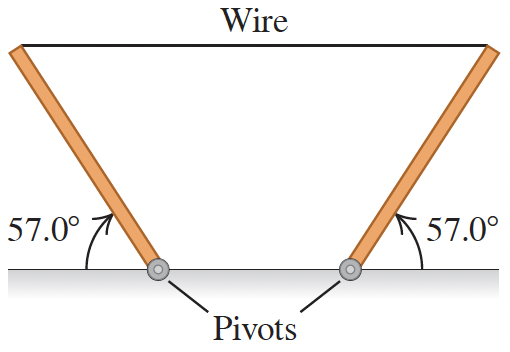
\includegraphics[width=0.5\linewidth]{../figures/P15_53.png}
  \label{fig:P15_53}
\end{figure}

A \qty{5,00}{m}, \qty{0,732}{kg} wire is used to support two uniform \qty{235}{N} posts of equal length (\textbf{\autoref{fig:P15_53}}). Assume that the wire is essentially horizontal and that the speed of sound is \qty{344}{m \per s}. A strong wind is blowing, causing the wire to vibrate in its 5th overtone. What are the frequency and wavelength of the sound this wire produces?

\begin{figure}[ht]
  \centering
  \incfig[0.25]{F27_15_53}
  \caption{Fritlegemediagram}
  \label{fig:F27_15_53}
\end{figure}
\bigbreak
For at der kan være statisk ligevægt gælder det at
\[ 
  \sum \tau_{0} = 0
.\]
Altså har vi at
\begin{align*}
  0 &= w \cdot \cos \theta \left( \frac{L}{2} \right) - T \sin \theta L \\
  T \sin \theta L &= w \cos \theta \frac{L}{2} \\
  T &= \frac{1}{2} w \cot \theta \\
    &= \frac{1}{2} \cdot \qty{235}{N} \cot \ang{57,0} \\
    &= \qty{76,3}{N} 
.\end{align*}
For at finde den 5. overtone (6. harmonic) benyttes formlen
\[ 
f_6 = \frac{6}{2L} \sqrt{\frac{F}{\mu}}
.\]
Massen pr. længdeenhed findes ved simpel division som
\[ 
\mu = \frac{\qty{0,732}{kg}}{\qty{5,00}{m}} = \qty{0,1464}{\frac{kg}{m}} 
.\]
Og spændingen i snoren $F = T$. Altså kan kendte størrelser sættes ind i formlen som
\begin{align*}
  f_6 &= \frac{6}{2\cdot \qty{5,00}{m}} \sqrt{\frac{\qty{76,3}{N}}{\qty{0,1464}{\frac{kg}{m}} }} \\
      &= \qty{13,69}{Hz}
.\end{align*}
Denne frekvens tilsvarer frekvensen af den producerede lyd. Bølgelængden af lyden kan derfor findes som
\[ 
\lambda = \frac{v}{f} \implies \lambda = \frac{\qty{344}{\frac{m}{s}}}{\qty{13,69}{Hz}} = \qty{25,1}{m} 
.\]


\section*{Opg. 15.61}
A sinusoidal transverse wave travels on a string. The string has
length \qty{8,00}{m} and mass \qty{6,00}{g}. The wave speed is \qty{30,0}{m \per s}, and the wavelength is \qty{0,200}{m}.

\subsection*{(a)}
If the wave is to have an average power of \qty{50,0}{W}, what must be the amplitude of the wave?
\bigbreak
Vi har den generelle formel for den gennemsnitlige effekt for en sinusoidal bølge på en snor som
\[ 
P_{av} = \frac{1}{2}\sqrt{\mu F} \omega^2 A^2
.\]
I denne kan amplituden isoleres som
\begin{align*}
  2P_{av} &= \sqrt{\mu F} \omega^2 A^2 \\
  A &= \sqrt{\frac{2P_{av}}{\sqrt{\mu F}\omega^2}}
.\end{align*}
Kraften kan isoleres i formlen
\[ 
v = \sqrt{\frac{F}{\mu}}
.\]
som
\[ 
F = \mu v^2
.\]
Sættes dette ind bliver det samlede udtryk for amplituden
\begin{align*}
  A &= \sqrt{\frac{2P_{av}}{\sqrt{\mu^2 v^2} \omega^2}} \\
  &= \sqrt{\frac{2P_{av}}{\mu v \omega^2}}
.\end{align*}
Vinkelfrekvensen er relateret til frekvens som
\[ 
\omega = 2\pi f
.\]
Og frekvensen kan findes vha. bølgelænden $\lambda$ og bølgehastigheden $v$ som
\[ 
f = \frac{v}{\lambda}
.\]
Altså bliver vinkelfrekvensen
\[ 
\omega = 2\pi \frac{v}{\lambda} \implies \omega^2 = 4 \pi^2 \frac{v^2}{\lambda^2}
.\]
Det samlede udtryk for amplituden bliver altså
\[ 
A = \sqrt{\frac{P_{av} \lambda^2}{2\pi^2 \cdot \mu\cdot v^3}}
.\]
Sættes kendte størrelser ind fås
\[
  A = \sqrt{\frac{\qty{50,0}{W} \cdot (\qty{0,200}{m})^2}{2\pi^2 \cdot \frac{\qty{0,00600}{kg}}{\qty{8,00}{m}} \cdot \left( \qty{30,0}{\frac{m}{s}}  \right)^3}} =\qty{0,0707}{m} = \qty{7,07}{cm}  
.\]



\subsection*{(b)}
For this same string, if the amplitude and wavelength are the same as in part (a), what is the average power for the wave if the tension is increased such that the wave speed is doubled?
\bigbreak
Vi har at $P_{av} \sim v^3$. Altså gælder at hvis $v$ fordobles så bliver $P_{av}$ 8 gange størrere. Altså bliver den gennemsnitlige effekt
\[ 
P_{av} = 8\cdot \qty{50,0}{W} = \qty{400}{W} 
.\]


\section*{Opg. 15.62}
\begin{figure} [ht]
  \centering
  \caption{}
  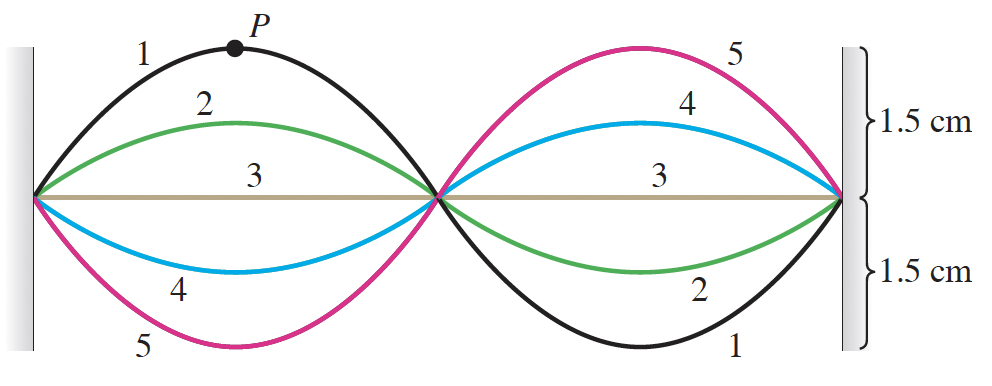
\includegraphics[width=0.5\linewidth]{../figures/P15_62.png}
  \label{fig:P15_62}
\end{figure}
A vibrating string \qty{50,0}{cm} long is under a tension of \qty{1,00}{N}. The results from five successive stroboscopic pictures are shown in \textbf{\autoref{fig:P15_62}}. The strobe rate is set at 5000 flashes per minute, and observations reveal that the maximum displacement occurred at flashes 1 and 5 with no other maxima in between.

\subsection*{(a)}
Find the period, frequency, and wavelength for the traveling waves on this string.
\bigbreak
Der bliver taget 5000 billeder i minutet og fra billede 1 til billede 5 ($\frac{1}{2}$ svingning) er der 4 billeder. Altså er der 8 billeder på en hel svingning. Derfor må frekvensen være
\[ 
f = \frac{\qty{5000}{min^{-1}}}{8\cdot \qty{60}{\frac{s}{min}} } = \qty{10,42}{Hz}  
.\]
Dette giver en periode på
\[ 
T = \frac{1}{f} = \frac{1}{\qty{10,42}{Hz}} = \qty{0,096}{s} 
.\]
Der er netop 1 bælgelængde over hele strengen og dermed har vi at $\lambda = \qty{50,0}{cm}$.


\subsection*{(b)}
In what normal mode (harmonic) is the string vibrating?
\bigbreak
Strengen vibrerer i sin 1. overtone og altså sin 2. \textit{harmonic} idet der netop er en hel bøl\-ge\-læng\-de på strengen (fundamentalfrekvensen ville tilsvare en halv bølgelængde over strengens længde).


\subsection*{(c)}
What is the speed of the traveling waves on the string?
\bigbreak
Bølgehastigheden $v$ er produktet af bølgelængden $\lambda$ og frekvensen $f$. Så
\[ 
v = \lambda f = \qty{0,5}{m} \cdot \qty{10,42}{Hz} = \qty{5,21}{\frac{m}{s}}  
.\]



\subsection*{(d)}
How fast is point $P$ moving when the string is in 

\subsubsection*{(i)}
position 1 and
\bigbreak
I position 1 oplever snoren sin maksimale forskydning og derfor må hastigheden her være $v_y = 0$.

\subsubsection*{(ii)}
position 3?
\bigbreak
Her oplever snoren sin maksimale hastighed $v_y = v_{y_{\text{max}}} = A \omega$. Altså er hastigheden her
\[ 
v_{y_{\text{max}}} = A\omega = A 2\pi f = \qty{1,5}{cm} \cdot 2\pi \cdot \qty{10,42}{Hz} = \qty{0,982}{\frac{m}{s}} 
.\]


\subsection*{(e)}
What is the mass of this string?
\bigbreak
Det vides at
\[ 
v = \sqrt{\frac{F}{\mu}} \implies \mu = \frac{F}{v^2}
.\]
Vi har tidligere fundet bølgehastigheden $v$ og spændingen i snoren $F = \qty{1,00}{N}$ er givet i opgaven. Altså kan massen pr. længde $\mu$ findes som
\[ 
\mu = \frac{\qty{1,00}{N}}{\left( \qty{5,21}{\frac{m}{s}}  \right)^2} = \qty{0,0369}{\frac{kg}{m}} 
.\]
Og snorens masse $m$ kan da findes som
\[ 
m = \mu \cdot l = \qty{0,0369}{\frac{kg}{m}} \cdot \qty{50,0}{cm} = \qty{0,0185}{kg} = \qty{18,5}{g}  
.\]



\section*{Opg. 15.69}
A large rock that weighs \qty{164,0}{N} is suspended from the lower end of a thin wire that is \qty{3,00}{m} long. The density of the rock is \qty{3200}{kg \per m^3}. The mass of the wire is small enough that its effect on the tension in the wire can be ignored. The upper end of the wire is held fixed. When the rock is in air, the fundamental frequency for transverse standing waves on the wire is \qty{42,0}{Hz}. When the rock is totally submerged in a liquid, with the top of the rock just below the surface, the fundamental frequency for the wire is \qty{28,0}{Hz}. What is the density of the liquid?
\bigbreak
Idet bølgen er ``fastspændt'' i begge ender må det i begge tilfælde gælde at bølgelænden $\lambda = 2L = \qty{6,00}{m}$. Bølgehastigheden for bølgen i luft kan nu findes som
\[ 
v_{air} = f_{air}\lambda = \qty{42,0}{Hz} \cdot \qty{6,00}{m} = \qty{252}{\frac{m}{s}} 
.\]
Vi har også at
\[ 
v_{air} = \sqrt{\frac{F}{\mu}} \implies \mu = \frac{F}{v_{air}^2}
.\]
Sættes værdier ind kan massen pr. længde $\mu$ findes som
\[ 
\mu = \frac{\qty{164,0}{N}}{\left( \qty{252}{\frac{m}{s}}  \right)^2} = \qty{0,00258}{\frac{kg}{m}} = \qty{2,58e-3}{\frac{kg}{m}} 
.\]
Bølgehastigheden i væsken kan findes som ovenfor
\[ 
v_{l} = f_l \lambda = \qty{28,0}{Hz} \cdot \qty{6,00}{m} = \qty{168}{\frac{m}{s}} 
.\]
Og denne må være lig
\[ 
v_l = \sqrt{\frac{F-B}{\mu}} \implies B = F- v_l^2 \cdot \mu
.\]
Sættes kendte størrelser ind kan størrelsen af opdriften findes som
\[ 
B = \qty{164,0}{N} - \left( \qty{168}{\frac{m}{s}}  \right)^2 \cdot \qty{2,58e-3}{\frac{kg}{m}} = \qty{91,2}{N}
.\]
Størrelsen af opdriftskraften er også givet ved følgende formel
\[ 
B = \rho V g \implies \rho = \frac{B}{Vg}
.\]
Stenens volumen kan findes som
\begin{align*}
  m &= \frac{F}{g} = \frac{\qty{164,0}{N}}{\qty{9,80}{\frac{m}{s^2}} } = \qty{16,7}{kg} \\ 
  V &= \frac{m}{\rho} = \frac{\qty{16,7}{kg}}{\qty{3200}{\frac{kg}{m^3}} } = \qty{0,00522}{m^3} 
.\end{align*}
Og altså kan densiteten af væsken findes som
\[ 
\rho = \frac{\qty{91,2}{N}}{\qty{0,00522}{m^3} \cdot \qty{9,80}{\frac{m}{s^2}} } = \qty{1782,78}{\frac{kg}{m^3}} = \qty{1,78e3}{\frac{kg}{m^3}} 
.\]



\end{document}
